\parindent=1cm %красная строка
\begin{center}
		
		\section{Защита личной переписки}
		
\end{center}

Принимая во внимание большое число угроз, рассмотрим существующие правовые и фактические способы обеспечения секретности тайны связи.
\subsection{Способы защиты и ответственность в правовом аспекте}

Уже упомянутый Федеральный закон <<Об информации, информационных технологиях и о защите информации>>   вводит дисциплинарную, гражданско-правовую, административную или уголовную ответственность за   нарушение интересов и прав лиц, пострадавших от разглашения информации ограниченного доступа или любого другого неправомерного использования данной информации.   Подробности защиты тайны связи в России и мире рассмотрены в пункте 1.1 <<Понятия в правовом аспекте>>
%LITER: http://www.consultant.ru/cons/cgi/online.cgi?req=doc&base=LAW&n=221952&fld=134&dst=100144,0&rnd=0.40247948281489154#07281395619440368
%определяет набор правовых, организационных и технических мер,  целью которых является  защита информации от неправомерного доступа, модификации, блокирования, копирования и распространения. Также вводится ответственность за правонарушения в сфере информационных технологий и защиты информации.
\subsection{Обзор существующего ПО для защиты переписки  и его анализ}
Далее  рассмотрены существующие способы защиты тайны переписки в интернете с помощью существующего ПО, проведен детальный анализ и выбраны оптимальные средства для конкретных задач, т.е. оптимального баланса простоты использования, доступности и надёжности. Также рассмотрены методы защиты от угроз описанных  в пункте 2.2. 
\\


\textbf{Использование доверенного безопасного  ПО. } В первую очередь, для защиты частной переписки необходимо убедиться в использовании оригинальных программных продуктов, поставляемых надёжными поставщиками. В качестве критериев надёжности можно выбрать:
\begin{itemize}
	\item Популярность. Если продукт находится на рынке достаточно долго, имеет хорошие отзывы и нет известных инцидентов компрометации данного продукта, то такой продукт можно считать <<надёжным>>. 
	\item Получение из оригинальных источников. Используемый продукт необходимо получать только от доверенного поставщика, т.е. ПО должно быть получено от официального дистрибьютора и/или из доверенного источника (официальный сайт, репозиторий).	
	\item Проверка на оригинальность. Для защиты от реверс-инжиниринга и/или внедрения модификации в исполнимый файл или исходный код, если продукт распространяется в таком виде, необходимо использовать валидацию полученного     продукта с помощью хэш-функций, например MDA-5, SHA-256. Такой подход используется как для проприетарного    (пакет Office от Microsoft), так и для open-source ПО (wine, transmission, vim). В противном случае возможно изменение ПО для превращения в кейлоггер или аналогичную программу слежения. \\
\end{itemize}


\textbf{Средства анонимного или шифрованного общения: мессенджеры, ремейлеры, сетевые средства}. Анонимные оверлейные сети -- это сети, работающие поверх уже существующей и работающей сети. Рассмотрим такие примеры таких сетей:

\textbf{Tor, луковая маршрутизация}. Анонимная оверлейная сеть, использующая принцип <<луковой маршрутизации>> -- технология анонимного обмена информацией, использующая многократное шифрование и пересылку шифрованных данных через цепочку частных узлов. Идеи, связанные с ЛМ, впервые появились в конце 90-х годов XX века и активно применялись ВМС США. Основной принцип работы ЛМ и Tor как частного случая: маршрутизатор при старте сессии  передачи выбирает случайное число промежуточных маршрутизаторов, генерирует сообщение для каждого, шифруя их симметричным ключом и указывая для каждого маршрутизатора, какой маршрутизатор будет следующим на пути (структура, аналогичная односвязному списку); для получения симметричного ключа устанавливается начальное соединение с каждым промежуточным маршрутизатором и используется его открытый ключ; таким образом, передаваемые по сети сообщения имеют <<луковую>> структуру, где для получения доступа к содержимому сообщения необходимо поочередно <<снимать слои>> ; каждый маршрутизатор <<снимает один слой>>, получает предназначенные только ему указания маршрутизации (следующий прокси) и шифрованное сообщение, которое необходимо передать далее; последний маршрутизатор <<снимает последний слой>>, отправляет сообщение адресату. Таким образом формируется устойчивая сеть, где каждый прокси передает сообщения в любую сторону, наращивая слои шифрования при передаче ответного сообщения\cite{TOR1}. %LITER http://www.inf.uni-konstanz.de/dbis/teaching/ss03/internet-protocols/download/onion.pdf
%LITER http://cryptome.org/2014/08/onion-routing-security-2000.pdf
%GRAPH https://upload.wikimedia.org/wikipedia/commons/d/dc/Tor-onion-network.png
\begin{figure*}[h!]
	\centering{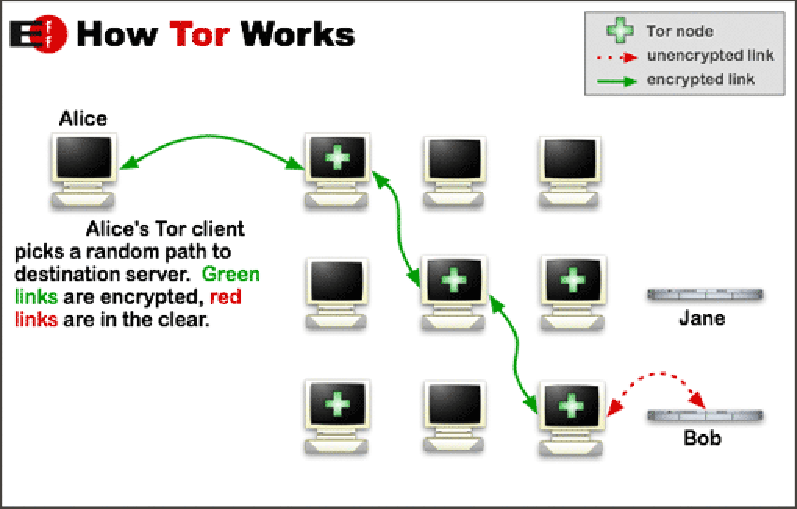
\includegraphics[scale=0.8]{HowToTor.pdf}}
	\caption{ Принцип работы луковичных сетей, описанный создателями Tor.}
\end{figure*} 

Преимущества Tor и луковой маршрутизации:высокая степень несвязности сети, прямо зависящая от кол-ва участвующих прокси; возможность работы даже при наличии скомпрометированных узлов, если только вся сеть не стоит из таких узлов; сочетание Tor и других средств шифрования и анонимности позволяет бороться с PRISM\cite{TOR2}.  %LITER https://www.pgpru.com/novosti/2013/prismprotivtor


Недостатки: отсутствие защиты от анализа синхронизации в слабонагруженных сетях, отсутствие защиты   от анализа данных, проходящих через выходные узлы, т.к. оператор может получить доступ к данным через сниффинг, если только не используется конечная криптография типа SSL/TSL; уязвимости к атакам MITM,  по времени, по сторонним каналам, глобальному пассивному наблюдению;  %LITER https://www.pgpru.com/faq/anonimnostjobschievoprosy#h37444-7
%LITER https://webcourse.cs.technion.ac.il/236349/Spring2014/ho/WCFiles/2011-01-2.report.pdf
%LITER https://arstechnica.com/information-technology/2013/09/snoops-can-identify-tor-users-given-enough-time-experts-say/
%LITER https://www.freehaven.net/anonbib/topic.html
ошибки  в программной реализации; на последнем узле цепи Tor возможна деанонимизация отправителя или модификация отправляемого сообщения;  при работе с сетью  к сообщениям пользователя может добавляться техническая информация, полностью либо частично раскрывающая отправителя. %LITER https://xakep.ru/2014/10/27/tor-russia/

\textbf{Чесночная маршрутизация, I2P}.I2P --  проект, начатый с целью создания анонимной компьютерной сети, работающей поверх сети интернет. Создатели проекта разработали свободное программное обеспечение (ПО), позволяющее реализовать сеть, работающую поверх сети интернет. Такая сеть является оверлейной, устойчивой к отключению узлов, шифрованной и анонимной к определению IP-адресов. Внутри сети возможно размещение любого сервиса или службы: файлообменник, электронную почту, форум, чат, VoIP) при полном сохранении анонимности сервера. I$ ^{2} $P допускает построение одноранговых сетей типа BitTorrent, Kad, Gnutella. %LITER https://geti2p.net/ru/get-involved/develop/licenses 
Сеть является самоорганизующейся и распределённой, используется модифицированный DHT Kademlia, при этом сеть хранит хешированные адреса узлов сети, зашифрованные AES-протоколом IP-адреса и публичные ключи шифрования, при этом соединения по Network database тоже зашифрованы.	Сеть предоставляет приложениям транспортный механизм для анонимной и защищённой пересылки сообщений друг другу. %LITER Анонимность в сети Интернет // КомпьютерПресс : журнал. — 2010. — № 9.
Благодаря библиотеке Streaming lib реализована  доставка пакетов  в первоначально заданной последовательности без ошибок, потерь и дублирования, что даёт возможность использовать в сети I2P IP-телефонию, интернет-радио, IP-телевидение, видеоконференции и другие потоковые протоколы и сервисы \cite{I2P1}. %LITER Денис Колисниченко. Анонимность и безопасность в Интернете: от "чайника" к пользователю. — БХВ-Петербург, 2011. — С. 44, 46, 47. — 240 с. — ISBN 978-5-9775-0363-1.
Внутри сети  существует автономный каталог сайтов, электронные библиотеки,торрент-трекеры. Также существуют шлюзы для доступа в сеть I2P непосредственно из Интернета, созданные  для пользователей, которые  не могут установить на компьютер программное обеспечение <<Проекта Невидимый Интернет>>. Внутри I2P реализованы механизмы шифрования, P2P (peer to peer )-архитектура, перемены посредников (хопы).

Преимущества: сеть изначально проектировалась с предположением скомпрометированности  всех промежуточных узлов, \cite{I2P2} %LITER Adrian Crenshaw. Darknets and hidden servers: Identifying the true IP/network identity of I2P service hosts // In the Proceedings of Black Hat 2011. — Washington, DC, 2011.
весь трафик шифруется от отправителя до получателя с использованием четырёх уровней шифрования (сквозное, чесночное, туннельное,  шифрование транспортного уровня), добавляется небольшое случайное количество случайных байт; все пакеты зашифровываются на стороне отправителя и расшифровываются только на стороне получателя, при этом никто из промежуточных участников обмена не имеет возможности перехватить расшифрованные данные и никто из участников не знает, кто на самом деле отправитель и кто получатель; сеть устойчива к потере даже значительного (более 50\%) числа узлов и попыткам внешнего анализа.

Недостатки: уязвимость к подмене узлов, при которой  злоумышленник заменяет рабочие узлы на скомпрометированные; перехвата туннелей; атака методом исключения, при которой злоумышленник последовательным перебором может установить, какие маршрутизаторы используются конкретным пользователем; %LITER https://xakep.ru/2014/09/04/i2p-secrets/
Sybil attack, позволяющая без захвата контроля над узлом закрыть доступ узлам сети 	к определённой информации; низкая скорость доступа, для синхронизации с сетью требуется примерно час.

\textbf{JonDo}. ПО, предоставляющее доступ к цепочке прокси-серверов, напоминающее Tor. В отличии  от  Tor, где ноду может создать любой участник, JonDo опирается на помощь отдельных организаций и группировок. К недостаткам относятся все уязвимости Tor, низкая скорость доступа, сильно ограниченное число нод.

\textbf{Ремейлеры} представляют собой серверы, пересылающие сообщения электронной почты по указанному адресу. Делятся на псевдонимные и анонимные. Последние делятся на ремейлеры шифропанков, MixMaster, MixMinion. При использовании псевдо-анонимного ремейлера, его оператор знает адрес электронной почты, который необходим для получения ответа на письмо. Тайна связи полностью зависит от оператора, который может стать жертвой угроз, шантажа или социальной инженерии. Преимуществом псевдо-анонимных ремейлеров является их юзабилити, за которое пользователь расплачивается меньшей защищённостью. Анонимные ремейлеры обеспечивают гораздо более высокую секретность, но при этом они и сложнее в использовании. Их операторы не могут знать, какие данные пересылаются через них, а поэтому нет гарантии своевременной доставки сообщения, которое может и вовсе затеряться.%LITER https://www.pgpru.com/forum/anonimnostjvinternet/kakajatomrachnajaatmosferavokrugremejjlerovremailers
В обмен на высокое время ожидания анонимные ремейлеры достаточно надёжно скрывают от посторонних глаз реальный адрес и содержимое сообщения. 
\begin{itemize}
	\item Ремейлеры шифропанков удаляют из полученных писем всю информацию, которая может быть использована для идентификации отправителя, и пересылают письмо на указанный адрес. Чаще всего используется PGP-шифрование, возможно создание цепочки таких ремейлеров.
	\item MixMaster. Требуют установки и более совершенны, чем прошлый тип, т.к отправляемые сообщения всегда константного размера, что делает невозможной отслежу по размерам.
	\item MixMinion.  Стандарт реализации третьего типа протокола анонимной пересылки электронной почты, может отсылать и принимать анонимные сообщения электронной почты, основан на пересылаемых защищённых одноразовых блоках. %LITER https://gnunet.org/sites/default/files/minion-design.pdf
\end{itemize}
Ремейлеры также имеют ряд уязвимостей и недостатков: тэговая атака, атака на выходные узлы, DDoS, путь доставки сообщений не всегда является оптимальным.

\textbf{Стеганография}. Способ тайной передачи информации путем сохранения в тайне самого факта передачи информации. В отличие от криптографии, которая скрывает содержимое тайного сообщения, стеганография скрывает сам факт его существования. Как правило, сообщение будет выглядеть как что-либо иное, например, как изображение, статья, список покупок, письмо или судоку. Стеганографию обычно используют совместно с методами криптографии, таким образом, дополняя её. Термин введен  в конце XV века монахом Иоганном Тритемием в трактате <<Steganographia>>, зашифрованном под магическую книгу. Криптография защищает содержание сообщения,  стеганография --  сам факт наличия каких-либо скрытых посланий.  Существует множество аналоговых методов стеганографии, однако в контексте данной работы рассматриваются только цифровые методы.  \textbf{Цифровая стеганография} — направление  стеганографии, основанное на сокрытии и/или внедрении дополнительной информации в цифровые объекты, вызывая при этом   искажения этих объектов. Как правило, данные объекты являются мультимедиа-объектами (изображения, видео, аудио, текстуры 3D-объектов) и внесение искажений, находящихся вне порога чувствительности среднестатистического человека, не приводит к значительным изменениям этих объектов. Также, в оцифрованных объектах, первоначально имеющих аналоговую природу, всегда присутствует шум квантования. Существующие алгоритмы цифровой стеганографии:
\begin{itemize}
	\item Сетевая стеганография, основанная на использовании особенностей работы сетевых протоколов передачи данных, когда части отдельных пакетов заменяются битами секретной информации. %LITER http://ijigroup.com/index.php?id=81
	\item Встраивание в изображение, при этом алгоритм работает непосредственно с цифровым сигналом (LSB), накладывает (fusion) изображение поверх существующего (цифровые водяные знаки), использование особенностей файлов (хранение в метаданных или неиспользуемых полях).
	\item Эхо-методы аудио-стеганографии, использующие неравномерные промежутки между эхо-сигналами для кодирования последовательности значений. 
\end{itemize}
Необходимо помнить, что если алгоритм  стеганографии или используемое ПО станут известны аналитику, анализ может быть проведен за адекватное время, поэтому перед кодировкой сообщений их необходимо шифровать с помощью криптографии \cite{Steg}. %LITER https://www.alternet.org/story/11986/confounding_carnivore%3A_how_to_protect_your_online_privacy


В целом, стеганография является качественным методом для передачи небольших (по сравнению с файлом, в который происходит встраивание) текстовых сообщений или мультимедиа объектов. Однако, стеганография не имеет широкой популярности и имеет уязвимости: атака на основании известного заполненного контейнера,  на основании известного встроенного сообщения,  на основании выбранного встроенного сообщения, на основании известного пустого контейнера, на основании выбранного пустого контейнера, на основании известной математической модели контейнера или его части.
%GRAPH steganography
\begin{figure*}[h!]
	\centering{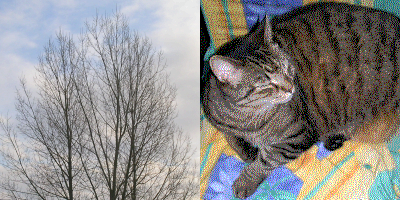
\includegraphics[scale=0.8]{steganography.png}}
	\caption{ Фото кота, вставленное и полученное из фото с деревом, пример использования fusion-алгоритмов.}
\end{figure*} 

\textbf{Мессенджеры}. Наиболее классическая и очевидная область применения существующих наработок в области защиты тайны связи, т.к. содержат преимущественно частную переписку, подвергающуюся анализу со стороны злоумышленников и государств.  Ниже рассмотрены самые популярные мировые мессенджеры (РФ в целом следует европейским трендам)  \cite{PopApp}. %LITER https://superfamilyprotector.com/blog/en/most-popular-messaging-apps-2018/
%LITER https://www.similarweb.com/blog/worldwide-messaging-apps
%LITER https://akket.com/raznoe/73783-top-10-samyh-populyarnyh-messendzherov-v-rossii-kotorymi-polzuyutsya-vse-rossiyane.html
%LITER https://www.rbc.ru/technology_and_media/18/01/2016/569cddd29a794722c534df2c
%GRAPH https://www.rbc.ru/technology_and_media/18/01/2016/569cddd29a794722c534df2c PopularMessage.png	
\begin{figure*}[h!]
	\centering{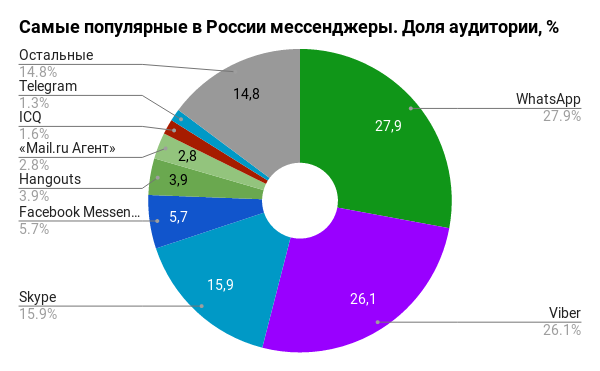
\includegraphics[scale=0.4]{PopularMessage.png}}
	\caption{Диаграмма популярности мессенджеров в РФ по данным РБК, 2017 год \cite{PopAppRus} .}
\end{figure*} 
\textbf{Viber}. Первый по популярности мессенджер  в РФ. В 2016 году Viber получил сквозное (end-to-end ) шифрование, однако подробности работы, например, симметричность или асимметричность, метод распределения ключей.  При этом через шифрование проходят как текстовые, так и мультимедийные объекты, пересылаемые в диалогах.ля этого каждый из клиентов использует открытый и закрытый ключ. Их генерирование осуществляется автоматически в момент установки программы на устройствах обеих сторон, что является потенциальной уязвимостью, так как ключи не уникальны для каждого диалога.%LITER http://allmessengers.ru/viber/shifrovanie
%LITER https://www.viber.com/ru/security/
Существует мнение, что <<поскольку и алгоритмы шифрования, и ключи шифрования, и уже расшифрованные сообщения находятся внутри софта мессенджера на конечном устройстве, доступ к любой информации у владельца мессенджера может быть>> и Viber не является в этом отношении исключением, кроме того <<Viber компрометируют себя функцией создания копий истории переписки>>  \cite{Viber}. %LITER https://www.kommersant.ru/doc/3379658
Более того, имел место инцидент со взломом одного из вспомогательных сервисов Viber Support в 2013 году группировкой <<Syrian Electronic Army>>. %LITER https://www.engadget.com/2013/07/23/viber-support-page-hacked-by-syrian-electronic-army/ 
В 2015, согласно Закону << О персональных данных>>, требующего хранения персональных данных россиян на территории РФ, Viber принял решения о переносе номеров телефонов и никнеймов на территорию РФ, предоставив доступ правоохранительным органам. Были высказаны опасения, что дата-центры могут быть атакованы злоумышленниками на территории РФ, что потенциально ведет к значительной утечке данных. %LITER http://www.the-village.ru/village/business/news/224095-viber-personal-data

\textbf{WhatsApp}. Второй по популярности мессенджер в РФ.  По состоянию на март 2015 года ежедневный объем трафика составлял 50 млрд. сообщений. %LITER https://vc.ru/5924-whatsapp-growth
WhatsApp использует модифицированный протокол XMPP, при установке создаётся аккаунт на сервере s.whatsapp.net, использующий номер телефона в качестве имени пользователя, порт под Android автоматически использует в качестве пароля MD5-хеш от изменённого идентификатора IMEI, а версия под iOS --  MD5-хеш от MAC-адреса.
%LITER https://github.com/venomous0x/WhatsAPI/
Из-за такого слабого алгоритма генерации пароля (MD5 содержит множество доказанных уязвимостей и коллизий %LITER https://tools.ietf.org/html/rfc6151
) и отсутствия шифрования, WhatsApp подвергался критике  \cite{WuzUp}. %LITER https://www.worldcrunch.com/tech-science/whatsapp-popular-free-messaging-service-puts-users-at-risk/whatsapp-smartphone-iphone-hacker-spam/c4s9533

С апреля 2016 мессенджер получил технологию сквозного шифрования. Шифрование распространяется на все типы сообщений: текст, фото, видео и голосовые сообщения. Шифрование также доступно в групповых чатах.%LITER https://blog.whatsapp.com/10000618/end-to-end-encryption
%LITER https://republic.ru/posts/66271	 
В  2017 года стало известно, что в системе шифрования сообщений был обнаружен бэкдор, позволяющий компании Facebook  скрытно изменять ключи шифрования и потребовать от приложения-отправителя перешифровать сообщения на новых ключах, а затем повторно отправлять их (при включённой настройке «Show Security Notifications» отправитель увидит уведомление о подобном факте после  перешифрования сообщений). Фактически эта функциональность позволяет серверам Facebook перехватывать и расшифровывать сообщения пользователей. Обнаруживший данную уязвимость исследователь  обратился в Facebook в 2016 году, но получил ответ, что данная функциональность известна авторам системы и является «ожидаемым поведением». Представитель компании пояснил, что возможность перешифровки сообщений необходима, так как часть пользователей часто меняет телефоны и сим-карты, а компания принимает меры, чтобы даже в таких случаях отправленные сообщения были доставлены получателям. %LITER https://www.theguardian.com/technology/2017/jan/13/whatsapp-design-feature-encrypted-messages
%LITER https://tobi.rocks/2016/04/whats-app-retransmission-vulnerability/
%LITER https://tobi.rocks/2017/01/whatsapp-vulnerability-bug-or-backdoor/
%LITER https://meduza.io/feature/2017/01/13/soobscheniya-v-whatsapp-mogut-prochitat-postoronnie-i-eto-ne-sobirayutsya-ispravlyat

\textbf{Telegram}. Мессенджер не входит в тройку самых популярных, однако реализует некоторые оригинальные технологии и породил много общественного резонанса. Итак, Telegram — кроссплатформенный мессенджер, позволяющий обмениваться сообщениями и медиафайлами многих форматов \cite{TG1} %LITER https://republic.ru/appheroes/telegram-novyy-messendzher-ot-pavla-durova-978067.xhtml
, использующий закрытую проприетарную  серверную часть и несколько версий открытых клиентов, доступных под лицензий GNU GPL. Telegram приобрел значительную популярность в связи с высказываниями владельца, Павла Дурова, о полной защищенности от прослушивания секретных  чатов данного мессенджера. %LITER https://vz.ru/news/2018/2/13/908109.html
%GRAPH https://ru.wikipedia.org/wiki/Telegram#%D0%A2%D0%B5%D1%85%D0%BD%D0%BE%D0%BB%D0%BE%D0%B3%D0%B8%D1%8F Telegram Popular
\begin{figure*}[h!]
	\centering{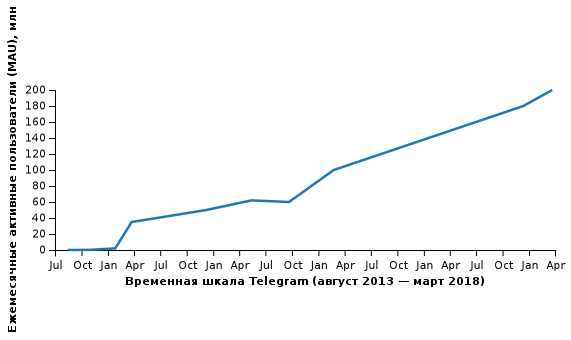
\includegraphics[scale=0.4]{TelegramPopular.png}}
	\caption{Рост популярности Telegram до и после начала конфликта  с РКН \cite{TG1}.}
\end{figure*} 

В основе коммуникации лежит протокол MTProto, предполагающий использование нескольких протоколов шифрования. 	 Для авторизации и аутентификации используются алгоритмы RSA-2048, DH-2048 для шифрования, при передаче сообщений протокола в сеть они шифруются AES с ключом, известным клиенту и серверу. Также применяются криптографические хеш-алгоритмы SHA-1 и MD5.  С 2013 года появился режим «секретных» чатов (Secret Chats).	Такой режим реализует шифрование, при котором только  отправитель и получатель обладают общим ключом (end-to-end), применяется  алгоритма AES-256 в режиме  Infinite Garble Extension для пересылаемых сообщений. Отличия данного режима работы от классического заключается в том, что сообщения не расшифровываются сервером, а только пересылаются через него, сами сообщения хранятся на устройствах в зашифрованном виде. Протокол допускает использование шифрования end-to-end с опциональной сверкой ключей, используется  протокол Диффи-Хэлмана для обмена 2048-битными RSA-ключами между двумя устройствами и ряд хеш-функций.
%GRAPH https://upload.wikimedia.org/wikipedia/commons/3/3e/MTProto_Cloud_Chats_scheme.png MTProto.png
\begin{figure*}[h!]
	\centering{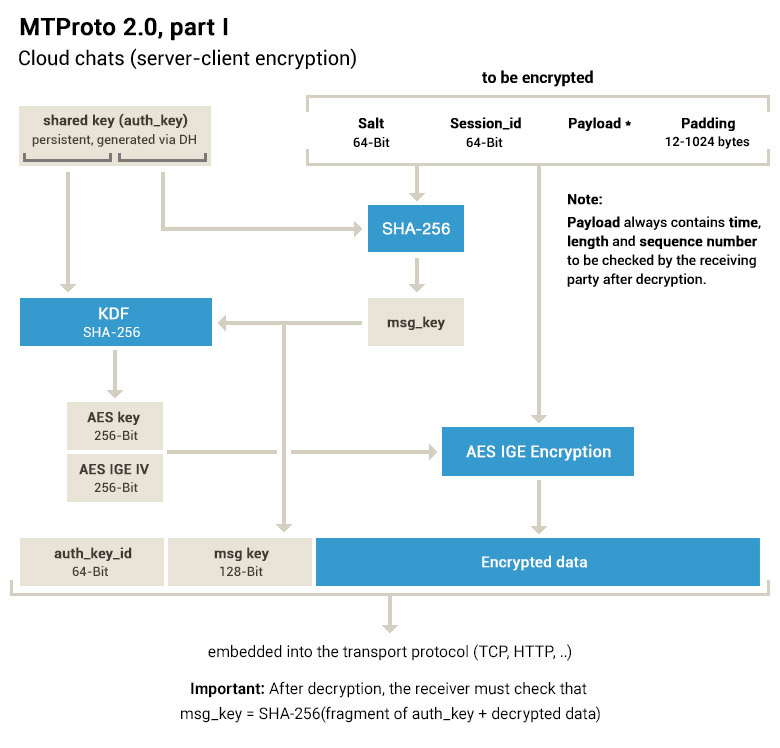
\includegraphics[scale=0.4]{MTProto.png}}
	\caption{Принцип работы протокола MTProto}
\end{figure*} 

В июне 2017 года Роскомнадзор  публично направил обращение Павлу Дурову с требованием предоставить информацию о компании для последующего внесения мессенджера Telegram в Реестр организаторов распространения информации в сети: полное и сокращенное наименование, страна регистрации, налоговый идентификатор и/или идентификатор в торговом реестре страны регистрации, адрес местонахождения, почтовый адрес, электронный адрес, доменное имя, электронный адрес администратора ресурса, провайдера хостинга и описание сервиса, предоставляемой услуги. %LITER https://www.vedomosti.ru/technology/articles/2017/05/16/690045-roskomnadzor-ugrozhaet-zakrit-telegram
После отказа предоставить данные, Дуров официально был предупрежден о возможности блокировки Telegram на территории РФ. %LITER https://www.rbc.ru/business/23/06/2017/594caae29a794703c5d3a4f4
Позже мессенлжеру было предъявлено требование предоставить ФСБ ключи для расшифровки обычных и секретных чатов, на что получили отказ, связанный с невозможностью предоставить ключи к секретным чатам, связанную с особенностями работы MTProto. С 16 апреля 2018 года РКН начал блокировку мессенджера на территории РФ.
%LITER https://ria.ru/society/20180411/1518373344.html
%LITER http://tass.ru/obschestvo/5121612
%LITER http://tass.ru/ekonomika/5129977
%LITER https://news.softodrom.ru/ap/b30424.shtml

Преимущества: высокий уровень анонимности, доступность в заблокированных странах, постоянное внедрение новых технологий передачи данных и защиты сообщений.

Недостатки: до 16 версий протокола была  возможность атаки повтором, состоящей в необходимости доверять серверу номера сообщений, что приводило к возможности повторной передаче сообщений злоумышленником и создавало возможность анализа ответов сервера и других абонентов; timing-атака, использующая  временной интервал между отправкой сообщения и приеме ответа об ошибке; по данным публикаций, протокол не имеет authenticated encryption и indistinguishability under chosen-ciphertext attack, что делает возможным две атаки:
\begin{itemize}
	\item Атака с увеличением длины сообщения. К сформированному шифротексту $ C=\{tags, y_{1}, y_{2}, ... , y_{l}\} $ , который дешифруется в сообщение $ X= \{tags,message,padding\} $ добавляется новый блок 128 бит, т.е принимаемый шифротекст принимает вид $ C'=\{tags, y_{1}, y_{2}, ... , y_{l}, r\} $, где $ r $ -- добавочный блок 128 бит. Сообщение расшифровывается как $ X'= \{tags,message,padding'\} $, в котором $  padding' =  \{padding, padding^{*}\}$ и длинна$  padding' $ больше длины блока. Т.к длинна $ padding $ не проверяется, дешифрование пройдет успешно. Для предотвращения данного типа атаки необходимо лишь проверять длину блока padding, в случае превышения допустимого размера необходимо прекращать дешифрование сообщения.
	\item Атака с изменением последнего шифрованного блока. В сформированном шифротексте $ C=\{tags, y_{1}, y_{2}, ... , y_{l}\} $, дешифруемом в сообщение $ X=  \{tags,message,padding\} $, изменяется последний блок и принимаемое сообщение  $ C $ принимает вид $ C'=\{tags, y_{1}, y_{2}, ... , y_{l-1}, r\} $. Таким образом, измененное сообщение расшифровывается как    $ X'= \{tags,message',padding'\} $ и длина $ padding' $ равна длине $ padding(p) $. С вероятностью $ 2^{-32} $ дешифрованное сообщение совпадает с оригинальным. Для предотвращения  такого типа атаки, необходимо добавить тег проверки padding в заголовки отправляемого сообщения \cite{TG2}. %LITER https://nourbakhsh.ir/wp-content/uploads/2015/11/jakobsen-master-thesis-telegram.pdf\\
	
\end{itemize}


По итогам обзора существующего ПО, рекомендуется использовать стеганографию для отправки небольших текстовых сообщений и мультимедиа, I$ ^{2} $P для анонимных форумов и хостингов  или одноранговых сетей типа BitTorrent и Telegram (как только будет решен конфликт с РКН или при условии вне РФ) для повседневных коммуникаций и аудиосвязи через интернет.

\subsection{Защита от основных видов угроз в частном секторе} 
Далее будут рассмотрены методы защиты от основных угроз существующих в частном секторе и рассмотренных в пункте 2.2.

\textbf{SpyWare}. Если угроза со стороны SpyWare становится более чем назойливой, существует ряд методов для борьбы с ними. Среди них программы, разработанные для удаления или блокирования внедрения SpyWare, также как и различные советы пользователю, направленные на снижение вероятности попадания SpyWare в систему. В случае значительной степени инфицированности ОС SpyWare наиболее действенным способом борьбы является сохранение данных пользователя (необходимо убедиться, что данные не заражены) и полная переустановка ОС. Также можно выделить методы по предотвращению заражения устройства: использование файрволов и прокси-серверов для блокировки доступа к сайтам, известным как распространители spyware, использование hosts-файла, препятствующего возможности соединения компьютера с сайтами, известным как распространители spyware, скачивание программ только из доверенных источников (предпочтительно с веб-сайтов производителя), поскольку некоторые spyware могут встраиваться в дистрибутивы программ, использование антивирусных программ с максимально «свежими» вирусными базами. Т.к основной целью SpyWare является конфиденциальная информация, рекомендуется  использование  одноразовых паролей/двухфакторная аутентификация, использование систем проактивной защиты, использование виртуальных клавиатур (неактуально для ПО, делающего снимки экрана).

\textbf{MITM}. Основное решение -- использование стойкого шифрования между клиентом и сервером. В таком случае сервер может идентифицировать себя посредством предоставления цифрового сертификата, после чего между пользователем и сервером устанавливается шифрованный канал для обмена конфиденциальными данными. Но в этом случае возникает зависимость от самого сервера и выбора им метода шифрования. Другим вариантом защиты от некоторых видов MITM-атак является полный отказ от использования открытых Wi-Fi-сетей для работы с личными данными. Хорошую защиту дают некоторые плагины для браузеров. Например, <<HTTPS Everywhere>> или <<ForceTLS>>, которые самостоятельно устанавливают защищенное соединение всякий раз, когда эта опция доступна на стороне сервера. %LITER https://www.kaspersky.ru/blog/chto-takoe-chelovek-poseredine/740/

\textbf{Защита от атак на криптографические протоколы}. Детальный разбор всех средств защиты от существующих методов атак лежит далеко за границами данной работы, тем не менее ниже рассмотрены самые распространенные способы борьбы с угрозами из пункта 2.2.

Для защиты от атаки подменой используется привязка ключей к обоим контрагентам, идентификаторы которых передаются друг другу в шифрованном, обычно, хэш-функцией, виде. Для защиты от replay attack используется  построение криптостойкой системы аутентификации. Основная идея состоит в том, что каждая сессия аутентификации использует оригинальные параметры (ключи) : метка времени создания ключа, случайное число, одноразовые коды. Защита от атак с использованием специально подобранных текстов подразумевает включение случайных чисел в post-get запросы и использование протоколов с нулевым разглашением -- интерактивный криптографический протокол, позволяющий одной из взаимодействующих сторон  убедиться в достоверности какого-либо утверждения (обычно математического), не имея при этом никакой другой информации от второй стороны. Для защиты от known-key атаки обеспечивают независимость  между различными применяемыми ключами, достигаемой с помощью протоколов совместной выработки ключа, не позволяющего ни одной стороне узнать ключ по существующим данным до выработки совместного ключа. И наконец, для зашиты от атак, использующих особенности специфику данного протокола, необходимо провести анализ существующей архитектуры, найти <<бутылочные горлышки>>, использовать более надёжные генераторы случайных чисел, передавать данные с хэш-<<солью>>. \\


\subsection{Реализация собственного программного продукта} 


В качестве собственного ПО для защиты тайны переписки предлагается реализация модифицированного алгоритма BLOWFISH -- криптографический алгоритм, реализующий блочное симметричное шифрование с переменной длиной ключа, разработанный  Брюсом Шнайером в 1993 году и представляющий собой сеть Фейстеля -- один из методов построения блочных шифров, в котором сеть состоит из ячеек, называемых ячейками Фейстеля; на вход каждой ячейки поступают ключ и данные, а на выходе каждой ячейки получают изменённые данные и изменённый ключ, при этом все ячейки однотипны  и  сама  сеть представляет собой определённую итерированную  (многократно повторяющуюся) структуру; ключ выбирается в зависимости от алгоритма шифрования/дешифрования, меняется при переходе между ячейками. При шифровании/ дешифровании выполняются одни и те же операции, а отличается только порядок ключей. 

Алгоритм выбран по причине простоты реализации, сравнительно высокой устойчивости и высокой скорости работы. Алгоритм выполнен на быстрых и простых для CPU операциях: сложение, подстановка и XOR (исключающее или) \cite{BF1}.

\textbf{Описание алгоритма}. Алгоритм состоит из двух частей: расширение ключа и шифрование данных. На этапе расширения ключа исходный ключ (длиной до 448 бит) преобразуется в 18 32-битовых подключей и в 4 32-битных S-блока, содержащих 256 элементов. Общий объём полученных ключей равен $ ( 18 + 256 * 4 ) * 32 = 33344   $ бит, т.е  $ 4168 $ байт.

Параметры алгоритма: секретный ключ K от 32 до 448 бит, 32-битные  таблицы $ S_{1} - S_{4}$, каждая по 225 элементов длиной; 32-битные шифрующие ключи $ P_{1}-P_{18} $.

Функция F(x), приминающая на вход блок в 32 бита и совершающая преобразование: 1.32-битный блок делится на четыре 8-битных блока $ X_{1}...X_{4} $, каждый из которых -- индекс массива таблицы замен $ S_{1} - S_{4}$. 2. Значения $ S_{1}[X_{1}] $ и $ S_{2}[X_{2}] $ складываются по модулю $ 2^{32} $, складываются по модулю 2 c $ S_{3}[X_{3}] $ и складываются также с $ S_{4}[X_{4}] $. 3. Результат этих операций  и есть значение $ F(x) $.


Алгоритм шифрования 64-битного блока с известным массивом P и F(x). Blowfish представляет собой Сеть Фейстеля, состоящую из 16 раундов. Алгоритм шифрования блока  X размером 64 бит выглядит следующим образом: 1.Разделение входного блока  X на 2 32-битных блока $ L_{0}, R_{0} $. 2. Для $ i=1;16 $: $ L_{i}=L_{i-1}+P_{i}; R_{i}= R_{i-1}+F(L_{i}) $. 3. После 16 раунда $ L_{16},R_{16} $ меняются местами, к получившимся блокам прибавляются $ P_{17}, P_{18} $. 4. Выходной блок Y = конкатенации $ L_{17},R_{17} $.

\textbf{Непосредственно алгоритм} разделен на 2 этапа:

1. Подготовительный — формирование ключей шифрования по секретному ключу. 
\begin{itemize}
	\item Инициализация массивов P и S при помощи секретного ключа K : 1.Инициализация $ P_{1} - P_{18} $ фиксированной строкой, состоящей из шестнадцатеричных цифр мантиссы числа Пи (могут быть выбраны любые другие значения:цифры числа e, RAND-таблицы или биты с выхода генератора случайных чисел );2.Производится операция XOR над $ P_{1} $ с первыми 32 битами ключа K и т.д. Если ключ $ K $ короче, то он накладывается циклически.
	\item Шифрование ключей и таблиц замен.  1.Алгоритм шифрования 64-битного блока, используя инициализированные ключи $ P_{1} - P_{18} $ и таблицу замен $ S_{1} - S_{4}$, шифрует 64-битную нулевую (0x0000000000000000) строку. Результат записывается в $ P_{1}, P_{2} $. 2. $ P_{1}, P_{2} $шифруются изменёнными значениями ключей и таблиц замен. Результат записывается в $ P_{3}, P_{4} $. 3. Шифрование продолжается до изменения всех ключей$ P_{1} - P_{18} $ и таблиц замен  $ S_{1} - S_{4}$.
\end{itemize}

2. Шифрование текста полученными ключами и F(x), с предварительным разбиением на блоки по 64 бита. Если невозможно разбить начальный текст точно на блоки по 64 бита, используются различные режимы шифрования для построения сообщения, состоящего из целого числа блоков. Суммарная требуемая память 4168 байт.

Дешифрование происходит аналогично, только  $ P_{1}-P_{18}  $ применяются в обратном порядке. 

\textbf{Криптостойкость}. Вероятность появления слабого S-блока равна   $ 2^{-15} $. Невозможно заранее определить, является ли ключ слабым. Проводить проверку можно только после генерации ключа.  Криптостойкость можно настраивать за счёт изменения количества раундов шифрования (увеличивая длину массива P) и количества используемых S-блоков. При уменьшении используемых S-блоков возрастает вероятность появления слабых ключей, но уменьшается используемая память. Адаптируя Blowfish для 64-битной архитектуры, можно увеличить количество и размер S-блоков (а следовательно и память для массивов P и S), а также усложнить F(x), причём для алгоритма с такой функцией F(x) невозможны вышеуказанные атаки. Известно, что вариант Blowfish с уменьшенным количеством раундов является уязвимым к атаке на основе открытых текстов на сравнительно слабых ключах. Реализации Blowfish с 16 раундами шифрования не подвержены подобным атакам \cite{BF2}.

Исходный код ПО доступен по адресу Github.com/Coursework/Source, в качестве средств реализации выбран язык C\# и фреймворк .Net 4.5. Такой выбор обусловлен доступностью в C\# встроенных средств для работы с AES протоколом и генераторами случайных чисел, использование .Net значительно облегчает портабельность кода и исполнимых файлов между Windows, Linux и Mac.
\newpage